Graphs have become increasingly important structures for representing and understanding complex structures in a wide range of applications.
In computational biology, graph models of protein molecules are used to mine frequent substructural motifs\cite{Huan2005}. In chemical informatics, graphs are used to model the molecular structure of chemical compounds. Graphs are also used in diverse fields such as pattern recognition, computer vision, social networks and so on. Such applications require that graph queries are solved efficiently.

Deciding whether a graph contains another graph is called the \textit{subgraph isomorphism problem}. That is, a subgraph isomorphism exist between two graphs if there exists one-to-one mapping between the smaller graph and a subgraph of the larger graph such that edge the adjacencies are preserved. Testing for subgraph isomorphism for an $n$-node graph in an $m$-node larger graph is a combinatorial matching with $m^n$ possibilities, hence is expensive. Therefore for a given query, evaluating a database for subgraph  isomorphism by individually testing each graph  in the database is inefficient.  In fact, the subgraph isomorphism problem is known to be NP-complete\cite{np-complete}. In  many 
cases, the graph database is also very large. This makes it necessary to build a framework to facilitate efficient graph search.

%\begin{figure}
%\centering
%\epsfig{file=images/typical_subgraph_query.eps, height=2.5in, width=2.5in}
%\caption{Subgraph isomorphism query}
%\label{fig:fig101}
%\end{figure}


\begin{figure}
\centering
%& -shell-escape -enable-write18
\documentclass{standalone}
\usepackage{tikz}
\usetikzlibrary{external}
%\tikzexternalize
\usetikzlibrary{shapes,arrows}
\usepackage{caption}
\usetikzlibrary{matrix}
%\newcommand{mynodename}[#1]{\mathrm{#1}}\label{•} 
%\newcommand{mylabelleft}[#2]{label={[font=\fontsize{#1}{#1}\selectfont]above left:mynodename{#2}}}

\begin{document}
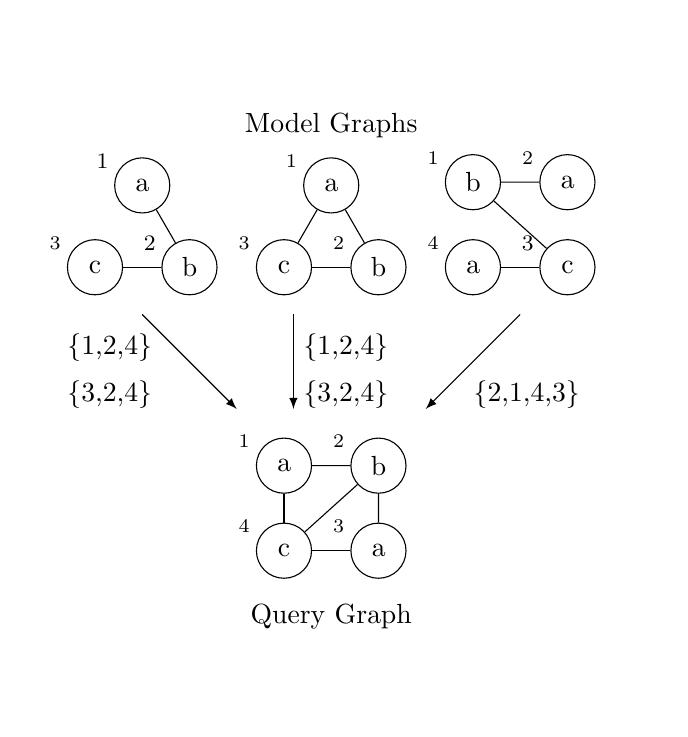
\begin{tikzpicture}[scale=1.2]
%[every node/.style={draw,circle}]
\tikzstyle{every node}=[draw,shape=circle,minimum size=0.7cm];
\tikzstyle{line} = [draw,-latex]
\colorlet{invisible}{white}
\colorlet{visible}{black}
%\tikzstyle{mylabelsfont=[font=\fontsize{7}{7}\selectfont,yshift=-.2cm];
%\tikzstyle{every label}=[text height=10pt];
\begin{scope}[shift={(0,-0.5)}] 
	\begin{scope}[yshift=0cm]% top row as a group
%	\draw[help lines] (-1,-6) grid (10,6);
	  \node (a) at (60:1cm) [label={[font=\fontsize{8}{8}\selectfont,yshift=-.2cm]above left:$1$}] {a};
	  \node (b) at (0:1cm)  [label={[font=\fontsize{8}{8}\selectfont,yshift=-.2cm]above left:$2$}] {b};
	  \node (c) at (0:0cm)  [label={[font=\fontsize{7}{7}\selectfont,yshift=-.2cm]above left:$3$}] {c};
	
	  \foreach \from/\to in {c/b,b/a}
	    \draw (\from) -- (\to);
	\end{scope}
	\begin{scope}[xshift=2cm]%top row middle
	  \node (a) at (60:1cm) [label={[font=\fontsize{7}{7}\selectfont,yshift=-.2cm]above left:$1$}] {a};
	  \node (b) at (0:1cm)  [label={[font=\fontsize{7}{7}\selectfont,yshift=-.2cm]above left:$2$}] {b};
	  \node (c) at (0:0cm)  [label={[font=\fontsize{7}{7}\selectfont,yshift=-.2cm]above left:$3$}] {c};
	
	  \node [draw=none] (query_label) at (0.5,1.5) {Model Graphs};% Model label
	  \foreach \from/\to in {c/b,b/a,c/a}
	    \draw (\from) -- (\to);
	\end{scope}
	\begin{scope}[xshift=4cm]%top row right
	  \node (a_1) at (0,0) [label={[font=\fontsize{7}{7}\selectfont,yshift=-.2cm]above left:$4$}] {a};
	  \node (b) at (0,.9)  [label={[font=\fontsize{7}{7}\selectfont,yshift=-.2cm]above left:$1$}] {b};
	  \node (c) at (1,0)   [label={[font=\fontsize{8}{8}\selectfont,yshift=-.2cm]above left:$3$}] {c};
	  \node (a_2) at (1,.9) [label={[font=\fontsize{7}{7}\selectfont,yshift=-.2cm]above left:$2$}] {a};
	
	  \foreach \from/\to in {a_1/c,c/b,b/a_2}
	    \draw (\from) -- (\to);
	\end{scope}
\end{scope}
\begin{scope}[shift={(0,0)}] % The arrow and bracket as a group
	\begin{scope}[shift={(0,-0.5)}]%just the arrows
		\path[line] (0.5,-0.5) -- (1.5,-1.5);
		\path[line] (2.1,-0.5) -- (2.1,-1.5);
		\path[line] (4.5,-0.5) -- (3.5,-1.5);
	\end{scope}
	\begin{scope}[shift={(0.5,-1.6)}]%annotations at left arrow
		\matrix (m)[matrix of nodes, column  sep=-1mm,color=visible,row  sep=-1mm, anchor=center,draw=none, nodes={rectangle,color=invisible,draw=none,text width = 2cm} ]{
\node [color=visible] {\{1,2,4\}};&\\
\node[color=visible]{\{3,2,4\}};& \\
};
	\end{scope}
	\begin{scope}[shift={(3.0,-1.6)}]%%annotations at middle arrow
	\matrix (m)[matrix of nodes, column  sep=-1mm,color=visible,row  sep=-1mm, anchor=center,draw=none,nodes={rectangle,color=invisible,draw=none,text width = 2cm} ]{
\node [color=visible] {\{1,2,4\}};&\\
\node[color=visible]{\{3,2,4\}};& \\
	};
	\end{scope}
	\begin{scope}[shift={(4.8,-1.6)}]%%annotations at right arrow
	\matrix (m)[matrix of nodes, column  sep=-1mm,color=visible,row  sep=-1mm, anchor=center,draw=none,nodes={rectangle,color=invisible,draw=none,text width = 2cm} ]{
\node [color=visible] {};&\\
\node[color=visible]{\{2,1,4,3\}};& \\
	};
	\end{scope}
\end{scope}

\begin{scope}[shift={(2,-3.5)}]%bottom row graph
  \node (a_3) at (1,0) [label={[font=\fontsize{7}{7}\selectfont,yshift=-.2cm]above left:$3$}] {a};
  \node (b) at (1,.9)  [label={[font=\fontsize{7}{7}\selectfont,yshift=-.2cm]above left:$2$}] {b};
  \node (c) at (0,0)   [label={[font=\fontsize{7}{7}\selectfont,yshift=-.2cm]above left:$4$}] {c};
  \node (a_4) at (0,.9) [label={[font=\fontsize{7}{7}\selectfont,yshift=-.2cm]above left:$1$}] {a};
  
  \node [draw=none] (query_label) at (.5,-.7) {Query Graph};% query graph label
  \foreach \from/\to in {a_3/c,a_3/b,c/b,c/a_4,b/a_4}
    \draw (\from) -- (\to);
    
\end{scope}
\end{tikzpicture}
\end{document}
\caption{Subgraph isomorphism query}
\label{fig:fig11}
\end{figure}


Messmer et al.\cite{messmer_bunke2000_ieee_kde} proposed an interesting so-called \textit{Network Algorithm, NA} to facilitate the retrieval of induced subgraph isomorphisms 
to a query graph from \textit{model graphs}. We refer to the Messmer et al.'s algorithm for constructing the network structure as \textit{NA method} in this paper and we call a graph stored in the graph database a \textit{model graph}.
This structure is constructed by decomposing graphs recursively, hence allowing the query can be processed in a divide and conquer fashion.

In this paper, we extend the \textit{NA method} to support \textit{non-induced subgraph isomorphism} queries.
Fig.\ref{fig:fig11} shows an example of a subgraph isomorphism query. We also reformulate the \textit{Network Algorithm} to increase the scalability of this method.
Our main contributions are as follows.

\begin{enumerate}
\item The \textit{network Method} originally only supports induced subgraph isomorphism query. We implement a version to process \textit{non-induced subgraph isomorphism} queries.
\item  In the Network Method, much of graph decomposition is performed on graphs at random potentially creating many graph fragments. We add a new recombining process after each decomposition which is active when more than a pair of  subgraphs result from the decomposition.  Recombining results in exactly  two larger graphs for each decomposition step, where possible.  As a consequence, we are able to reduce the potential  explosion in matchings. 
\item We formulate and implement  a  \textit{Fast Network Method}. The new algorithm decomposes only two connected subgraphs. 
%Random decomposition of graphs results in the generation of multiple graph fragments. The recombining step swaps nodes and  edges until only two graphs result from each decomposition.  
\end{enumerate}

We present experimental results where we compare our proposed algorithms with two well known subgraph isomorphism algorithms: Messmer et. al 's\cite{messmer} Network Algorithm that efficiently aggregates multiple graphs in a and VF2\cite{vf} Algorithm, based on sequential one-on-one graph isomorphism tests. 
%The results show that the proposed improvements result in an order of magnitude increase in scalability over the original  NA Method  for query graphs of up to 500 nodes to a database of 20,000 graphs.  Our method is particularly suited to larger query graphs or very larger graph databases.
